\section{Uniform Random Numbers}
Let $U$ be a uniform random variable between 0 and 1.
\begin{enumerate}
\item Generate $10^6$ samples of $U$ using a C program and save into a file called uni.dat .
\label{prob:uni_gen}
\\
\solution Download the following files and execute the  C program.
\begin{lstlisting}
	chapter2/codes/exrand.c
    chapter2/codes/coeffs.h
\end{lstlisting}

%
\item
Load the uni.dat file into python and plot the empirical CDF of $U$ using the samples in uni.dat. The CDF is defined as
\begin{align}
F_{U}(x) = \pr{U \le x}
\end{align}

\begin{lstlisting}
chapter2/codes/cdf_plot.py	
\end{lstlisting}
\begin{figure}[H]
\centering
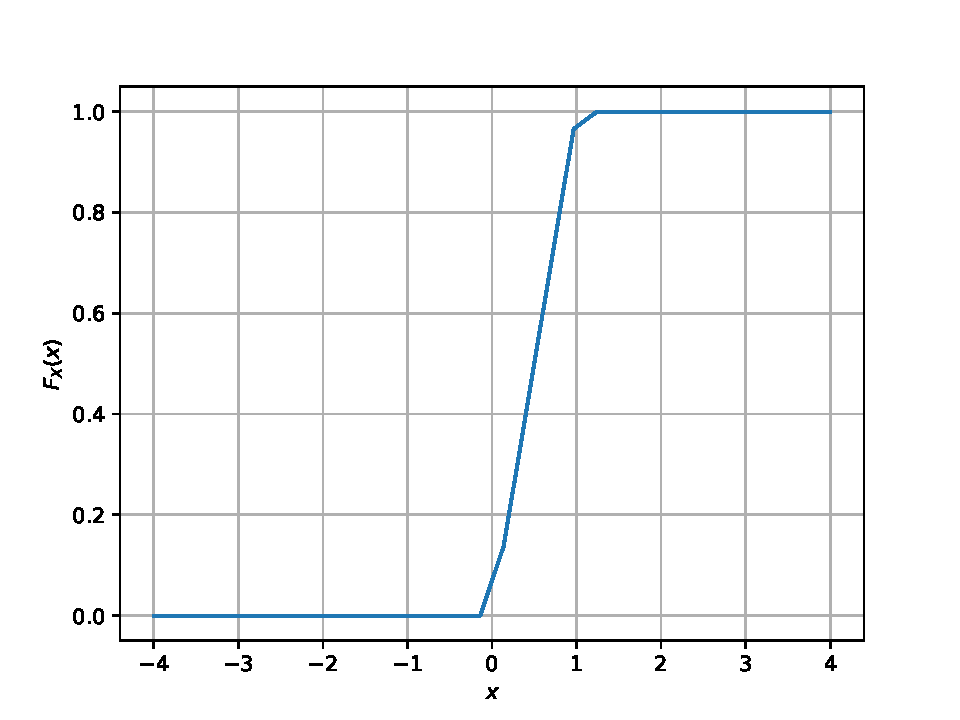
\includegraphics[width=\columnwidth]{chapter2/figs/uni_cdf.pdf}
\caption{The CDF of $U$}
\label{fig:uni_cdf}
\end{figure}
\item
Find a  theoretical expression for $F_{U}(x)$.\\
\solution
\begin{align} 
F_{U}(x) = \int_{-\infty}^{x} f_{U}(x)\,dx
\label{eq:pdf_to_cdf}
\end{align}
For the uniform random variable $U$, $f_{U}(x)$ is given by  
\begin{align}
	f_U(x) &= 
	\begin{cases}
	1 &  0 \le x \le  1
	\\
	0 & elsewhere
	\\
	\end{cases}
	\label{eq:uni_pdf}
\end{align}
Substituting \eqref{eq:uni_pdf} in \eqref{eq:pdf_to_cdf}, $F_U(x)$ is found to be
\begin{align}
	F_U(x) &= 
	\begin{cases}
	0 & x < 0
	\\	
	x & 0 \le x \le  1
	\\
	1 & x > 0
	\\
	\end{cases}
	\label{eq:uni_cdf}
\end{align}

\item
\label{prob:print_uni}
The mean of $U$ is defined as
%
\begin{equation}
E\sbrak{U} = \frac{1}{N}\sum_{i=1}^{N}U_i
\end{equation}
%
and its variance as
%
\begin{equation}
\text{var}\sbrak{U} = E\sbrak{U- E\sbrak{U}}^2 
\end{equation}

Write a C program to  find the mean and variance of $U$.\\
\solution The following code prints the mean and variance of $U$
\begin{lstlisting}
	chapter2/codes/mv.c
\end{lstlisting}
The output of the program is
\begin{lstlisting}
Uniform stats:
Mean: 0.500007
Variance: 0.083301
\end{lstlisting}

\item Verify your result theoretically given that
%
\begin{equation}
E\sbrak{U^k} = \int_{-\infty}^{\infty}x^kdF_{U}(x)
\end{equation}\\
\solution For a random variable $X$, the mean $\mu_X$ and variance $\sigma_X^2$ are given by
\begin{align}
	\label{eq:mean_exp}
	\mu_X &= E\sbrak{X} = \int_{-\infty}^{\infty}xdF_{U}(x) \\
	\label{eq:var_exp}
	\sigma_X^2 &= E\sbrak{X^2} - \mu_X^2 = \int_{-\infty}^{\infty}x^2dF_{U}(x) - \mu_X^2
\end{align}  
Substituting the CDF of $U$ from (2.1.3.3) in (2.1.5.2) and (2.1.5.3), we get
\begin{align}
	\label{eq:mean_uni}
	\mu_U &= \frac{1}{2} \\
	\label{eq:var_uni}
	\sigma_U^2 &= \frac{1}{12}
\end{align}  
which match with the values printed in problem 2.1.4
\end{enumerate}
\section{Central Limit Theorem}
\begin{enumerate}
\item
Generate $10^6$ samples of the random variable
%
\begin{equation}
X = \sum_{i=1}^{12}U_i -6
\end{equation}
%
using a C program, where $U_i, i = 1,2,\dots, 12$ are  a set of independent uniform random variables between 0 and 1
and save in a file called gau.dat\\
\solution Download the following files and execute the  C program.
\begin{lstlisting}
	chapter2/codes/rv.c
\end{lstlisting}
%
\item
Load gau.dat in python and plot the empirical CDF of $X$ using the samples in gau.dat. What properties does a CDF have?
\\
\begin{figure}[h!]
\centering
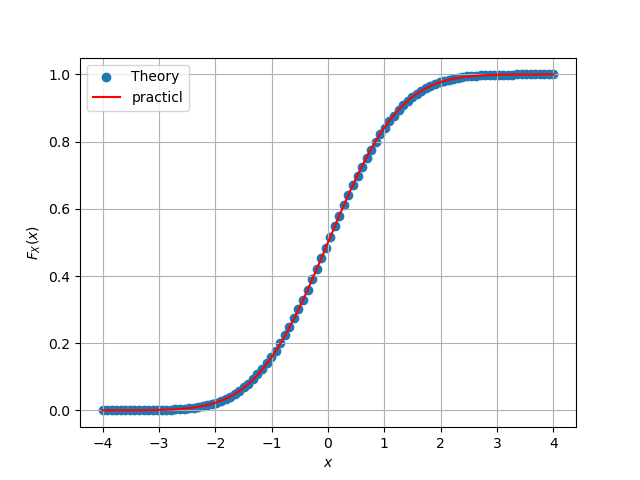
\includegraphics[width=\columnwidth]{chapter2/figs/gauss_cdf.png}
\caption{The CDF of $X$}
\label{fig:gauss_cdf}
\end{figure}
Let $X$ be a random variable (either continuous or discrete), then the CDF
of $X$ has the following properties
The CDF is a non-decreasing \\
The maximum of the CDF is when
\begin{eqnarray}
x = \infty: F_X(\infty) = 1
\end{eqnarray}
The minimum of the CDF is when
\begin{eqnarray}
x = -\infty: F_X(-\infty) = 0	
\end{eqnarray}
\item
Load gau.dat in python and plot the empirical PDF of $X$ using the samples in gau.dat. The PDF of $X$ is defined as
\begin{align}
p_{X}(x) = \frac{d}{dx}F_{X}(x)
\label{eq:cdf_to_pdf}
\end{align}
What properties does the PDF have?
\solution 
\begin{lstlisting}
	chapter2/codes/rv.c
\end{lstlisting}

\begin{figure}[h!]
\centering
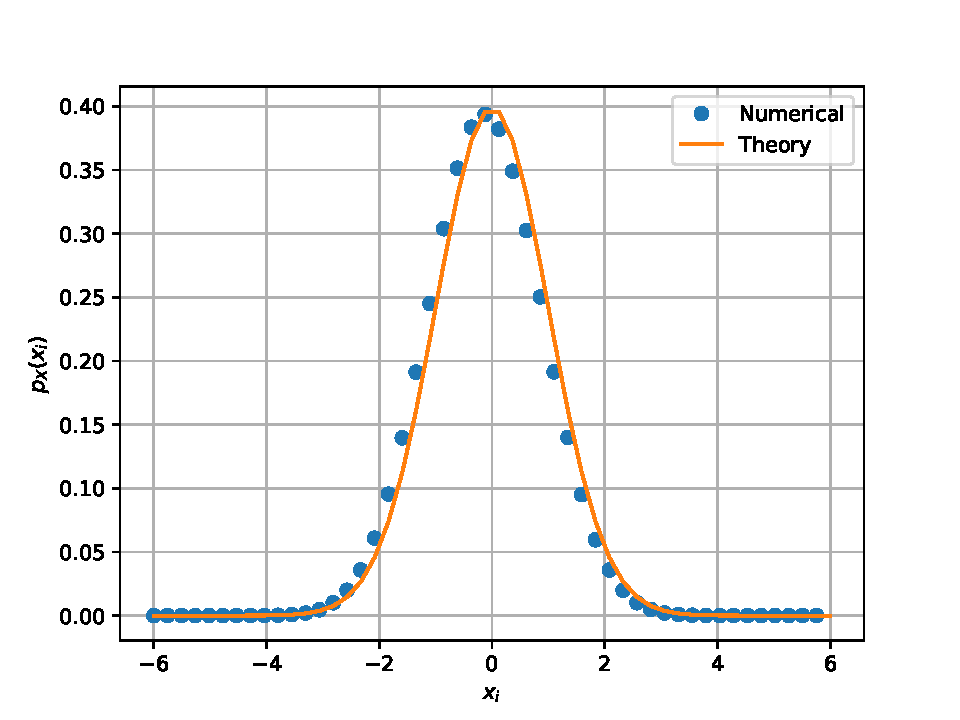
\includegraphics[width=\columnwidth]{chapter2/figs/gauss_pdf.pdf}
\caption{The PDF of $X$}
\label{fig:gauss_pdf}
\end{figure}

The properties of PDF are
\begin{eqnarray}
	f_X(x) \ge 0 \text{for all} X \in \mathbb{R} \\
	\int_{-\infty}^{\infty} f_X(x) \,dx = 1
\end{eqnarray}

\item Find the mean and variance of $X$ by writing a C program.
\solution The following code prints the mean and variance of $X$
\begin{lstlisting}
	chapter2/codes/mean.c
\end{lstlisting}
The output of the program is
\begin{lstlisting}
Gaussian stats:
Mean: 0.000294
Variance: 0.999561	
\end{lstlisting}
\item Given that 
\begin{align}
p_{X}(x) = \frac{1}{\sqrt{2\pi}}\exp\brak{-\frac{x^2}{2}}, -\infty < x < \infty,
\label{eq:gau_pdf}
\end{align}
repeat the above exercise theoretically.\\
\solution Substituting the PDF from \eqref{eq:gau_pdf} in \eqref{eq:mean_exp},
\begin{flalign}
	\mu_X &= \int_{-\infty}^{\infty} \frac{x}{\sqrt{2\pi}}\exp\brak{-\frac{x^2}{2}} \,dx&\\
	\intertext{Using}&\\
	\int x \cdot \exp \left( -a x^2 \right) \mathrm{d}x &= -\frac{1}{2a} \cdot \exp \left( -a x^2 \right)&\\
	\mu_X &= \frac{1}{\sqrt{2\pi}}\left[-\exp\brak{-\frac{x^2}{2}}\right]_{-\infty}^{\infty}&\\  
	\mu_X &= 0
\end{flalign}
Substituting $\mu_X$ and the PDF in \eqref{eq:var_exp} to compute variance,
\begin{flalign}
	\sigma_X^2 &= \int_{-\infty}^{\infty} \frac{x^2}{\sqrt{2\pi}}\exp\brak{-\frac{x^2}{2}} \,dx&\\ \nonumber
	\intertext{Substituting} t &= \frac{x^2}{2},&\\	
	\sigma_X^2 &= \frac{2}{\sqrt{\pi}} \int_{0}^{\infty} t^{\frac{1}{2}}\exp\brak{-t} \,dt&\\	\nonumber
	&= \frac{2}{\sqrt{\pi}} \int_{0}^{\infty} t^{\frac{3}{2}-1}\exp\brak{-t} \,dt&\\
	\intertext{Using the gamma function} \Gamma(x) &= \int_{0}^{\infty} z^{x-1} \cdot e^{-z} \, \mathrm{d}z \,&\\
	\sigma_X^2 &= \frac{2}{\sqrt{\pi}}\Gamma(\frac{3}{2})&\\	\nonumber
	&= \frac{2}{\sqrt{\pi}}\frac{\sqrt{\pi}}{2}&\\	\nonumber
	&=1	
\end{flalign}
%
\end{enumerate}


\section{From Uniform to Other}
\begin{enumerate}
%
\item
Generate samples of 
%
\begin{equation}
V = -2\ln\brak{1-U}
\end{equation}
%
and plot its CDF. \\
\solution
\begin{lstlisting}
	chapter2/2_3_cdf.py
\end{lstlisting}
\begin{figure}[H]
\centering
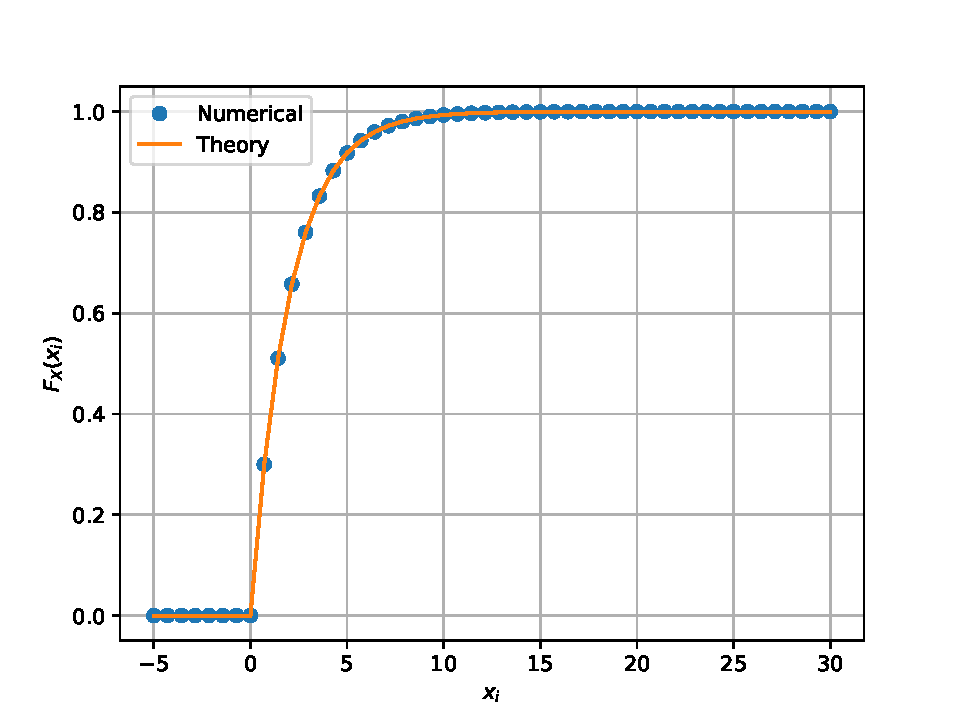
\includegraphics[width=\columnwidth]{chapter2/figs/log.pdf}
\caption{The CDF of $V$}
\label{fig:log_uni_cdf}
\end{figure}
\item Find a theoretical expression for $F_V(x)$.
\begin{flalign}
	F_V(x) &= P(V < x)&\\
	&= P(-2\ln\brak{1-U} < x)&\\
	&= P(U < 1 - e^{\frac{-x}{2}})&\\
	&= F_U(1 - e^{\frac{-x}{2}})
\end{flalign}
Using $F_U(x)$ defined in \eqref{eq:uni_cdf},
\begin{align}
	F_V(x) &=
	\begin{cases}
		0 & x < 0\\
		1 - e^{\frac{-x}{2}} & x \ge 0
	\end{cases}
\end{align} 
\end{enumerate}



\section{Triangular Distribution}
%
\begin{enumerate}
\item Generate 
	\begin{align}
		T = U_1+U_2
	\end{align}\\
\solution Download the following files and execute the  C program.
\begin{lstlisting}
chapter2/codes/tri.c
\end{lstlisting}
\item Find the CDF of $T$.\\
\solution 
\begin{lstlisting}
	chapter2/codes/tcdf.py
\end{lstlisting}
\begin{figure}[H]
\centering
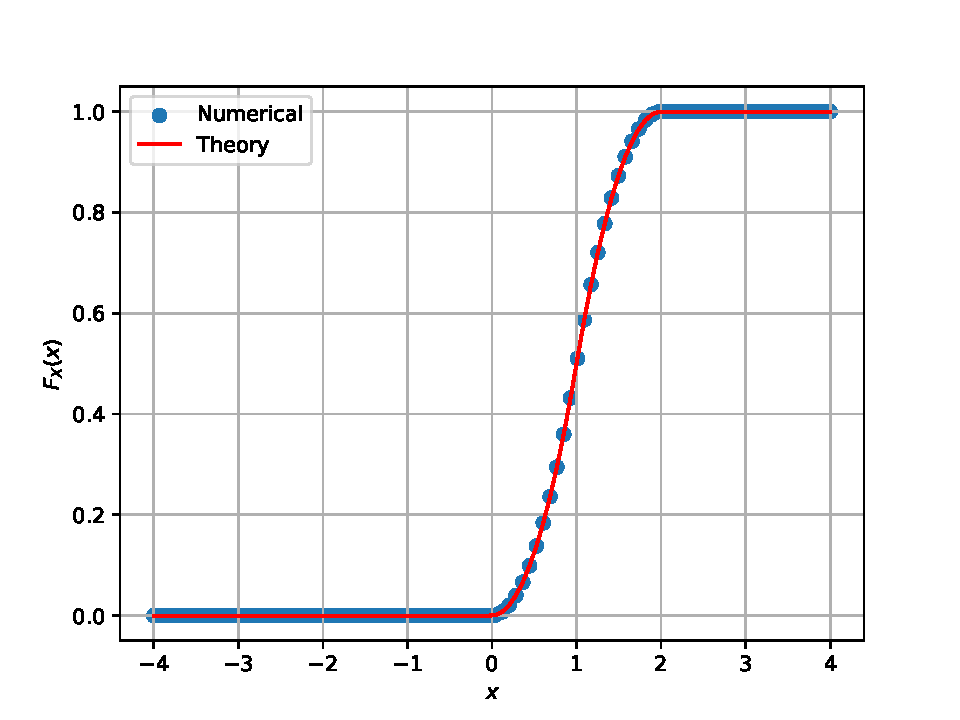
\includegraphics[width=\columnwidth]{chapter2/figs/triangle_cdf.pdf}
\caption{The CDF of $T$}
\label{fig:tri_cdf}
\end{figure}
\item Find the PDF of $T$.\\

\begin{lstlisting}
chapter2/codes/tdpf.py
\end{lstlisting}
\begin{figure}[H]
\centering
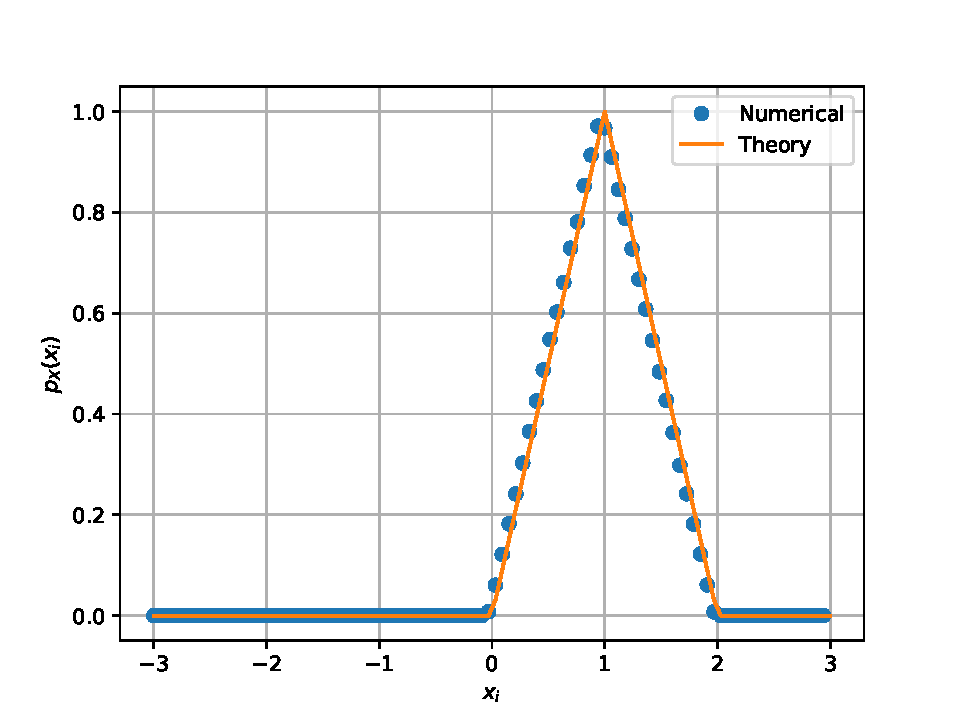
\includegraphics[width=\columnwidth]{chapter2/figs/triangle_pdf.pdf}
\caption{The PDF of $T$}
\label{fig:tri_pdf}
\end{figure}
\item Find the theoretical expressions for the PDF and CDF of $T$.\\
\solution Since $T$ is the sum of two independant random variables $U1$ and $U2$, the PDF of $T$ is given by
\begin{flalign}
	p_T(x) &= p_{U1}(x) \ast p_{U2}(x)
\end{flalign}
Using the PDF of $U$ from \eqref{eq:uni_pdf}, the convolution results in
\begin{align}
	p_T(x) &=
	\begin{cases}
		0 & x < 0\\
		x & 0 \le x \le 1\\
		2-x & 1 \le x \le 2\\
		0 & x > 2
	\end{cases}
	\label{eq:tri_pdf}
\end{align}
The CDF of $T$ is found using \eqref{eq:pdf_to_cdf} by replacing $U$ with $T$. Evaluating the integral for the piecewise function $p_T(x)$, 
\begin{align}
	F_T(x) &=
	\begin{cases}
		0 & x < 0\\
		\frac{x^2}{2} & 0 \le x \le 1\\
		2x-\frac{x^2}{2}-1 & 1 \le x \le 2\\
		1 & x > 2
	\end{cases}
\end{align}
\item Verify your results through a plot. \\
\solution The theoretical and numerical plots for the CDF and PDF of $T$ closely match in \figref{fig:tri_cdf} and \figref{fig:tri_pdf}
\end{enumerate}
